\documentclass[]{article}
\usepackage{lmodern}
\usepackage{amssymb,amsmath}
\usepackage{ifxetex,ifluatex}
\usepackage{fixltx2e} % provides \textsubscript
\ifnum 0\ifxetex 1\fi\ifluatex 1\fi=0 % if pdftex
  \usepackage[T1]{fontenc}
  \usepackage[utf8]{inputenc}
\else % if luatex or xelatex
  \ifxetex
    \usepackage{mathspec}
  \else
    \usepackage{fontspec}
  \fi
  \defaultfontfeatures{Ligatures=TeX,Scale=MatchLowercase}
\fi
% use upquote if available, for straight quotes in verbatim environments
\IfFileExists{upquote.sty}{\usepackage{upquote}}{}
% use microtype if available
\IfFileExists{microtype.sty}{%
\usepackage{microtype}
\UseMicrotypeSet[protrusion]{basicmath} % disable protrusion for tt fonts
}{}
\usepackage[margin=1in]{geometry}
\usepackage{hyperref}
\hypersetup{unicode=true,
            pdftitle={UVC datasets - exploring monitoring structure and herbivore assemblages},
            pdfborder={0 0 0},
            breaklinks=true}
\urlstyle{same}  % don't use monospace font for urls
\usepackage{color}
\usepackage{fancyvrb}
\newcommand{\VerbBar}{|}
\newcommand{\VERB}{\Verb[commandchars=\\\{\}]}
\DefineVerbatimEnvironment{Highlighting}{Verbatim}{commandchars=\\\{\}}
% Add ',fontsize=\small' for more characters per line
\usepackage{framed}
\definecolor{shadecolor}{RGB}{248,248,248}
\newenvironment{Shaded}{\begin{snugshade}}{\end{snugshade}}
\newcommand{\KeywordTok}[1]{\textcolor[rgb]{0.13,0.29,0.53}{\textbf{#1}}}
\newcommand{\DataTypeTok}[1]{\textcolor[rgb]{0.13,0.29,0.53}{#1}}
\newcommand{\DecValTok}[1]{\textcolor[rgb]{0.00,0.00,0.81}{#1}}
\newcommand{\BaseNTok}[1]{\textcolor[rgb]{0.00,0.00,0.81}{#1}}
\newcommand{\FloatTok}[1]{\textcolor[rgb]{0.00,0.00,0.81}{#1}}
\newcommand{\ConstantTok}[1]{\textcolor[rgb]{0.00,0.00,0.00}{#1}}
\newcommand{\CharTok}[1]{\textcolor[rgb]{0.31,0.60,0.02}{#1}}
\newcommand{\SpecialCharTok}[1]{\textcolor[rgb]{0.00,0.00,0.00}{#1}}
\newcommand{\StringTok}[1]{\textcolor[rgb]{0.31,0.60,0.02}{#1}}
\newcommand{\VerbatimStringTok}[1]{\textcolor[rgb]{0.31,0.60,0.02}{#1}}
\newcommand{\SpecialStringTok}[1]{\textcolor[rgb]{0.31,0.60,0.02}{#1}}
\newcommand{\ImportTok}[1]{#1}
\newcommand{\CommentTok}[1]{\textcolor[rgb]{0.56,0.35,0.01}{\textit{#1}}}
\newcommand{\DocumentationTok}[1]{\textcolor[rgb]{0.56,0.35,0.01}{\textbf{\textit{#1}}}}
\newcommand{\AnnotationTok}[1]{\textcolor[rgb]{0.56,0.35,0.01}{\textbf{\textit{#1}}}}
\newcommand{\CommentVarTok}[1]{\textcolor[rgb]{0.56,0.35,0.01}{\textbf{\textit{#1}}}}
\newcommand{\OtherTok}[1]{\textcolor[rgb]{0.56,0.35,0.01}{#1}}
\newcommand{\FunctionTok}[1]{\textcolor[rgb]{0.00,0.00,0.00}{#1}}
\newcommand{\VariableTok}[1]{\textcolor[rgb]{0.00,0.00,0.00}{#1}}
\newcommand{\ControlFlowTok}[1]{\textcolor[rgb]{0.13,0.29,0.53}{\textbf{#1}}}
\newcommand{\OperatorTok}[1]{\textcolor[rgb]{0.81,0.36,0.00}{\textbf{#1}}}
\newcommand{\BuiltInTok}[1]{#1}
\newcommand{\ExtensionTok}[1]{#1}
\newcommand{\PreprocessorTok}[1]{\textcolor[rgb]{0.56,0.35,0.01}{\textit{#1}}}
\newcommand{\AttributeTok}[1]{\textcolor[rgb]{0.77,0.63,0.00}{#1}}
\newcommand{\RegionMarkerTok}[1]{#1}
\newcommand{\InformationTok}[1]{\textcolor[rgb]{0.56,0.35,0.01}{\textbf{\textit{#1}}}}
\newcommand{\WarningTok}[1]{\textcolor[rgb]{0.56,0.35,0.01}{\textbf{\textit{#1}}}}
\newcommand{\AlertTok}[1]{\textcolor[rgb]{0.94,0.16,0.16}{#1}}
\newcommand{\ErrorTok}[1]{\textcolor[rgb]{0.64,0.00,0.00}{\textbf{#1}}}
\newcommand{\NormalTok}[1]{#1}
\usepackage{graphicx,grffile}
\makeatletter
\def\maxwidth{\ifdim\Gin@nat@width>\linewidth\linewidth\else\Gin@nat@width\fi}
\def\maxheight{\ifdim\Gin@nat@height>\textheight\textheight\else\Gin@nat@height\fi}
\makeatother
% Scale images if necessary, so that they will not overflow the page
% margins by default, and it is still possible to overwrite the defaults
% using explicit options in \includegraphics[width, height, ...]{}
\setkeys{Gin}{width=\maxwidth,height=\maxheight,keepaspectratio}
\IfFileExists{parskip.sty}{%
\usepackage{parskip}
}{% else
\setlength{\parindent}{0pt}
\setlength{\parskip}{6pt plus 2pt minus 1pt}
}
\setlength{\emergencystretch}{3em}  % prevent overfull lines
\providecommand{\tightlist}{%
  \setlength{\itemsep}{0pt}\setlength{\parskip}{0pt}}
\setcounter{secnumdepth}{0}
% Redefines (sub)paragraphs to behave more like sections
\ifx\paragraph\undefined\else
\let\oldparagraph\paragraph
\renewcommand{\paragraph}[1]{\oldparagraph{#1}\mbox{}}
\fi
\ifx\subparagraph\undefined\else
\let\oldsubparagraph\subparagraph
\renewcommand{\subparagraph}[1]{\oldsubparagraph{#1}\mbox{}}
\fi

%%% Use protect on footnotes to avoid problems with footnotes in titles
\let\rmarkdownfootnote\footnote%
\def\footnote{\protect\rmarkdownfootnote}

%%% Change title format to be more compact
\usepackage{titling}

% Create subtitle command for use in maketitle
\newcommand{\subtitle}[1]{
  \posttitle{
    \begin{center}\large#1\end{center}
    }
}

\setlength{\droptitle}{-2em}
  \title{UVC datasets - exploring monitoring structure and herbivore assemblages}
  \pretitle{\vspace{\droptitle}\centering\huge}
  \posttitle{\par}
  \author{}
  \preauthor{}\postauthor{}
  \date{}
  \predate{}\postdate{}


\begin{document}
\maketitle

\paragraph{Seychelles}\label{seychelles}

\begin{itemize}
\tightlist
\item
  Seychelles data are 7m radius point counts conducted at 21 reef sites
  in 1994, 2005, 2008, 2011, 2014, 2017.
\item
  Sites were stratified according to habitat (granite = 7, patch = 7,
  carbonate = 7) and management status (12 = fished, 9 = MPAs)
\item
  Reefs are the inhabited Seychelles islands, Mahe and Praslin
\item
  Useful papers describing dataset methods: Graham et al. 2015
  (Predicting climate-driven regime shifts\ldots{}, Nature)
\end{itemize}

Across all surveys, \texttt{37} herbivore species were recorded, which
are composed of:

\begin{verbatim}
##                  FG species
## 1 Herbivore Browser       5
## 2  Herbivore Grazer      15
## 3 Herbivore Scraper      17
\end{verbatim}

Scrapers dominated herbivore assemblages on both fished and protected
reefs, and browser biomass was slightly higher than grazer biomass after
1994 (i.e.~after bleaching). High variability in browser biomass
suggests that strong spatial variation in browser presence. This was
less true for scrapers, for which biomass may be high at all reef sites.
There was a weak protection effect apparent, with slightly higher
biomass of all feeding groups in protected sites.

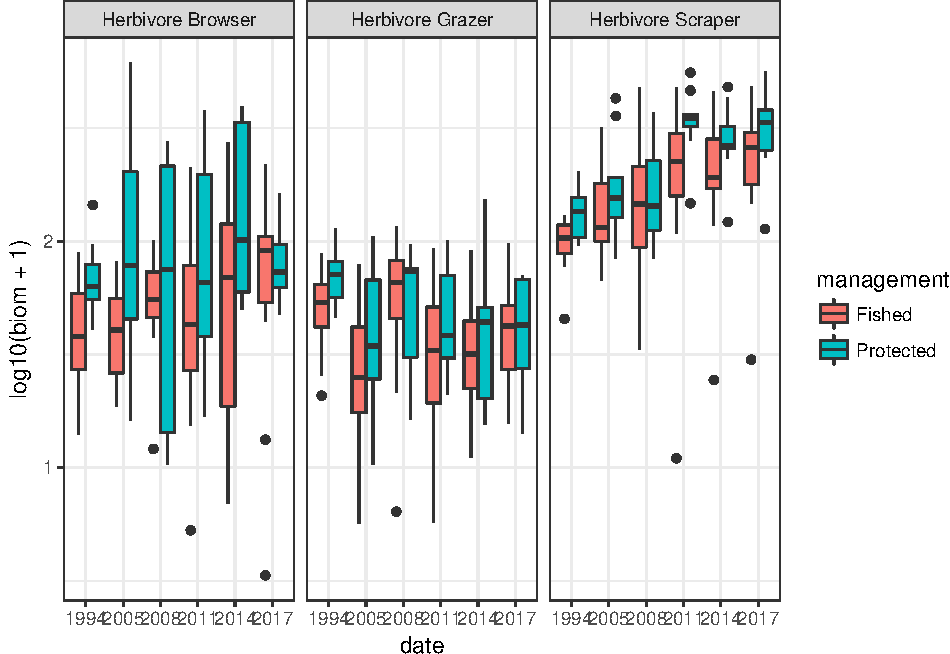
\includegraphics{UVC-datasets-explore_files/figure-latex/unnamed-chunk-3-1.pdf}

Grazer size distributions indicated high abundance of small-bodied
individuals. Scraper and browser sizes were more equitably distributed
across the size range. Scrapers had the largest body sizes, with some
individuals between 0.5-2 kg.

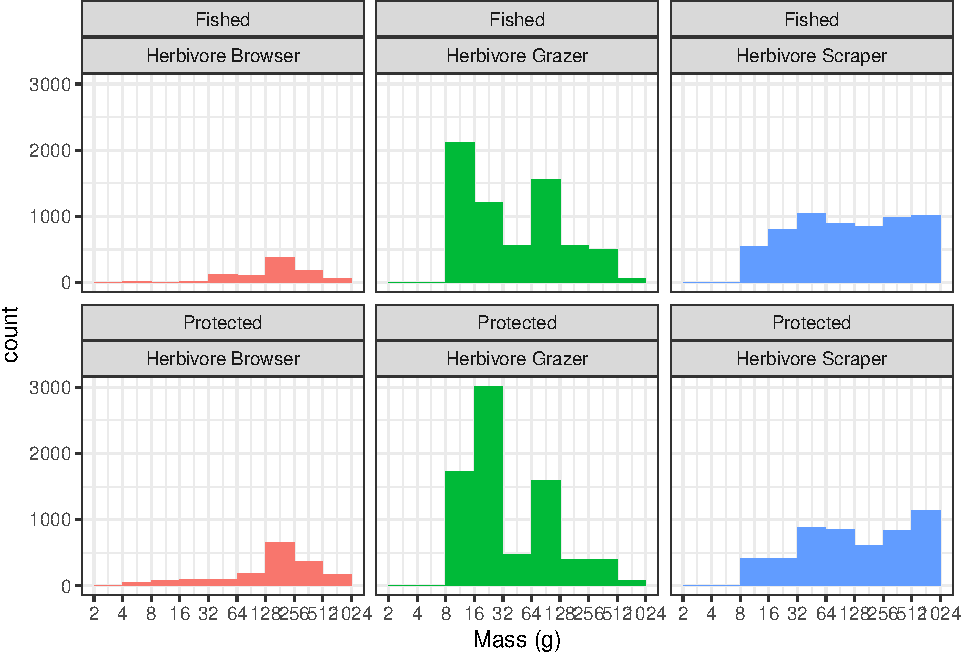
\includegraphics{UVC-datasets-explore_files/figure-latex/unnamed-chunk-4-1.pdf}

\textbf{Common herbivore species}

Considering common species as those that are high in abundance or
biomass (i.e.~mean biomass across UVC replicates at each site).

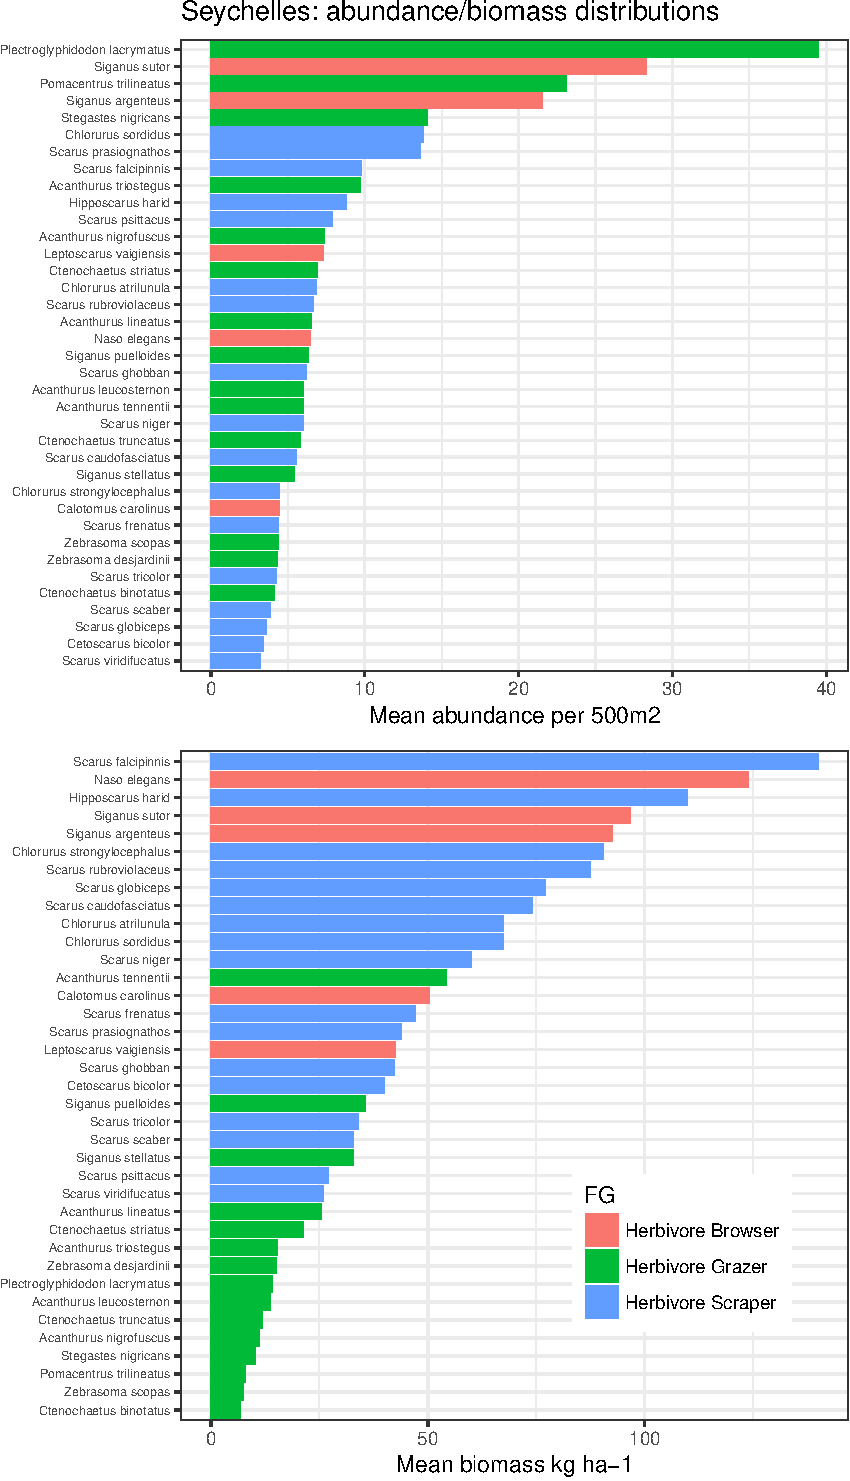
\includegraphics{UVC-datasets-explore_files/figure-latex/unnamed-chunk-5-1.pdf}

\paragraph{Maldives}\label{maldives}

\paragraph{GBR}\label{gbr}

\paragraph{Chagos}\label{chagos}

\emph{Exploring the data}

Total of 52 species, 5729 records, across 20 sites at 4 reefs, with
between 1-4 transects at each site

\begin{Shaded}
\begin{Highlighting}[]
\CommentTok{#From James script}
\CommentTok{# count number of unique species per functional group}
\KeywordTok{aggregate}\NormalTok{(species }\OperatorTok{~}\StringTok{ }\NormalTok{FG, chagos, }\ControlFlowTok{function}\NormalTok{(x) }\KeywordTok{length}\NormalTok{(}\KeywordTok{unique}\NormalTok{(x)))}
\end{Highlighting}
\end{Shaded}

\begin{verbatim}
##                  FG species
## 1 Herbivore Browser       5
## 2  Herbivore Grazer      22
## 3 Herbivore Scraper      25
\end{verbatim}

\begin{Shaded}
\begin{Highlighting}[]
\CommentTok{#From James script}
\NormalTok{## estimate size distribution by functional groups}
\KeywordTok{ggplot}\NormalTok{(chagos, }\KeywordTok{aes}\NormalTok{(}\KeywordTok{log}\NormalTok{(mass.g, }\DecValTok{2}\NormalTok{), }\DataTypeTok{fill=}\NormalTok{FG)) }\OperatorTok{+}\StringTok{ }\KeywordTok{geom_histogram}\NormalTok{(}\DataTypeTok{breaks=}\KeywordTok{c}\NormalTok{(}\DecValTok{1}\OperatorTok{:}\DecValTok{10}\NormalTok{)) }\OperatorTok{+}\StringTok{ }\KeywordTok{facet_wrap}\NormalTok{(management}\OperatorTok{~}\NormalTok{FG) }\OperatorTok{+}\StringTok{ }\KeywordTok{theme}\NormalTok{(}\DataTypeTok{legend.position=}\StringTok{'none'}\NormalTok{) }\OperatorTok{+}\StringTok{ }\KeywordTok{scale_x_continuous}\NormalTok{(}\DataTypeTok{breaks=}\KeywordTok{c}\NormalTok{(}\DecValTok{1}\OperatorTok{:}\DecValTok{10}\NormalTok{), }\DataTypeTok{labels=}\KeywordTok{c}\NormalTok{(}\DecValTok{2}\OperatorTok{^}\KeywordTok{c}\NormalTok{(}\DecValTok{1}\OperatorTok{:}\DecValTok{10}\NormalTok{))) }\OperatorTok{+}\StringTok{ }\KeywordTok{labs}\NormalTok{ (}\DataTypeTok{x=}\StringTok{'Mass (g)'}\NormalTok{)}
\end{Highlighting}
\end{Shaded}

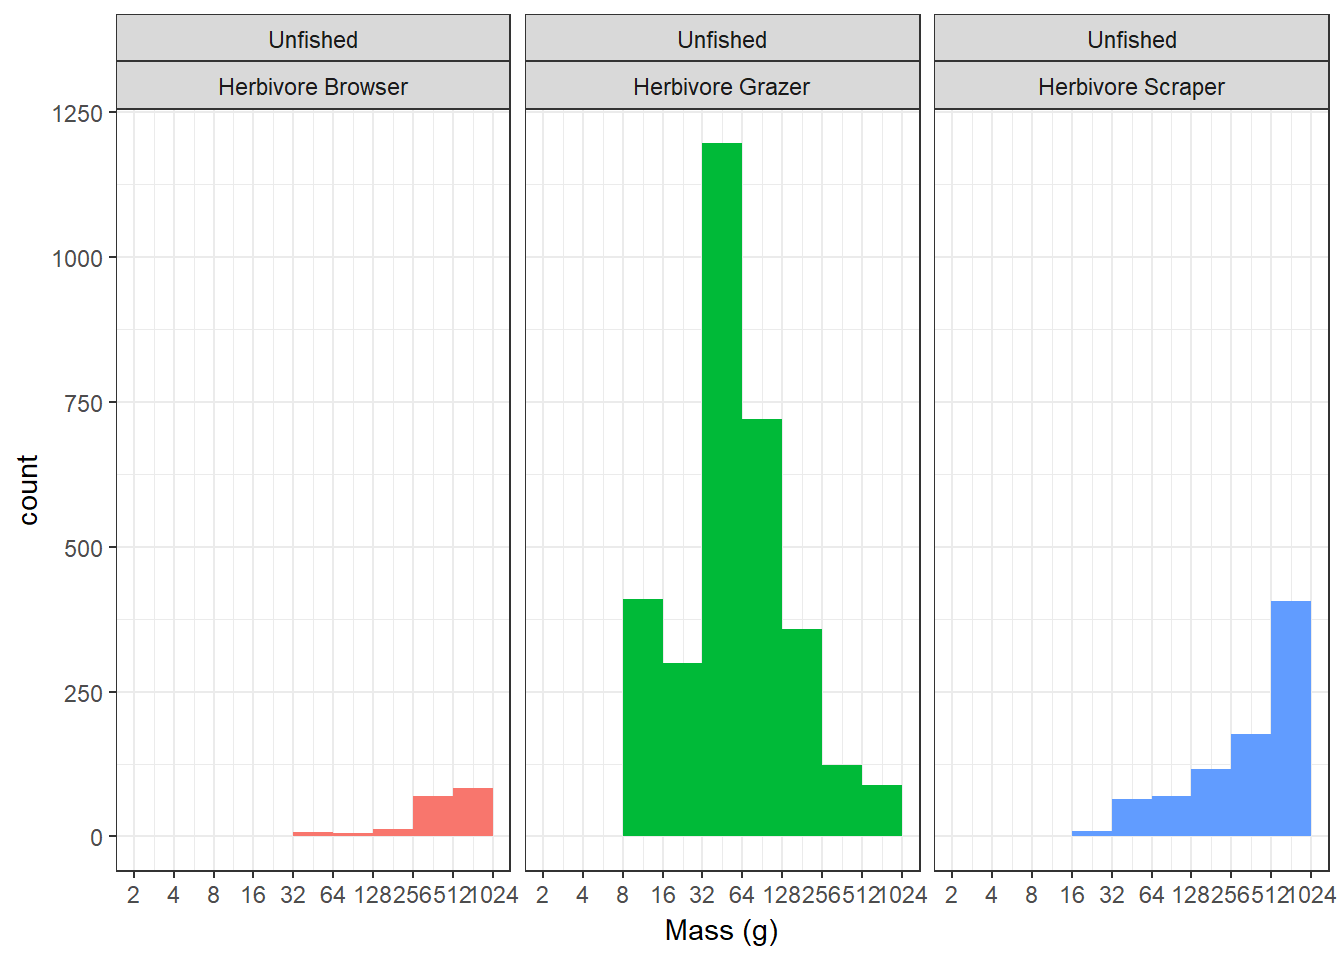
\includegraphics{UVC-datasets-explore_files/figure-latex/unnamed-chunk-10-1.pdf}

Now need to look at abundance and biomass of species and functional
groups across sites\ldots{}

\section{insert graphs on spp and FG abundance and biomass across sites,
what are the common
species?}\label{insert-graphs-on-spp-and-fg-abundance-and-biomass-across-sites-what-are-the-common-species}

\section{From James}\label{from-james}

\begin{Shaded}
\begin{Highlighting}[]
\NormalTok{## estimate mean abundance at site level, by species}
\NormalTok{abund <-}\StringTok{ }\NormalTok{chagos }\OperatorTok\StringTok{ }\KeywordTok{group_by}\NormalTok{(unique.id, site, species, FG) }\OperatorTok\StringTok{ }
\StringTok{        }\KeywordTok{summarise}\NormalTok{(}\DataTypeTok{abund =} \KeywordTok{sum}\NormalTok{(abundance.500m2)) }\OperatorTok\StringTok{ }\NormalTok{## total abundance per UVC}
\StringTok{        }\KeywordTok{group_by}\NormalTok{(species, FG) }\OperatorTok\StringTok{ }
\StringTok{        }\KeywordTok{summarise}\NormalTok{(}\DataTypeTok{abund =} \KeywordTok{mean}\NormalTok{(abund)) ## mean abundance per site}

\NormalTok{## estimate mean biomass at site level, by species}
\NormalTok{biom <-}\StringTok{ }\NormalTok{chagos }\OperatorTok\StringTok{ }\KeywordTok{group_by}\NormalTok{(unique.id, site, species, FG) }\OperatorTok\StringTok{ }
\StringTok{        }\KeywordTok{summarise}\NormalTok{(}\DataTypeTok{biom =} \KeywordTok{sum}\NormalTok{(biomass.kgha)) }\OperatorTok\StringTok{ }\NormalTok{## total biomass per UVC}
\StringTok{        }\KeywordTok{group_by}\NormalTok{(species, FG) }\OperatorTok\StringTok{ }
\StringTok{        }\KeywordTok{summarise}\NormalTok{(}\DataTypeTok{biom =} \KeywordTok{mean}\NormalTok{(biom)) ## mean biomass per site}

\NormalTok{g2<-}\KeywordTok{ggplot}\NormalTok{(abund[abund}\OperatorTok{$}\NormalTok{abund}\OperatorTok{<}\DecValTok{100}\NormalTok{,], }\KeywordTok{aes}\NormalTok{(}\KeywordTok{reorder}\NormalTok{(species,abund), abund, }\DataTypeTok{fill=}\NormalTok{FG)) }\OperatorTok{+}\StringTok{ }
\StringTok{  }\KeywordTok{geom_bar}\NormalTok{(}\DataTypeTok{stat=}\StringTok{'identity'}\NormalTok{) }\OperatorTok{+}\StringTok{ }
\StringTok{  }\KeywordTok{labs}\NormalTok{(}\DataTypeTok{y=}\StringTok{'Mean abundance per 500m2'}\NormalTok{, }\DataTypeTok{x=}\StringTok{''}\NormalTok{,}\DataTypeTok{title=}\StringTok{'Chagos: abundance/biomass distributions'}\NormalTok{) }\OperatorTok{+}
\StringTok{  }\KeywordTok{coord_flip}\NormalTok{() }\OperatorTok{+}\StringTok{ }\KeywordTok{theme}\NormalTok{(}\DataTypeTok{legend.position=}\StringTok{'none'}\NormalTok{, }\DataTypeTok{axis.text.y=}\KeywordTok{element_text}\NormalTok{(}\DataTypeTok{size=}\DecValTok{6}\NormalTok{))}

\NormalTok{g3<-}\KeywordTok{ggplot}\NormalTok{(biom[biom}\OperatorTok{$}\NormalTok{biom}\OperatorTok{<}\DecValTok{300}\NormalTok{,], }\KeywordTok{aes}\NormalTok{(}\KeywordTok{reorder}\NormalTok{(species,biom), biom, }\DataTypeTok{fill=}\NormalTok{FG)) }\OperatorTok{+}\StringTok{ }
\StringTok{  }\KeywordTok{geom_bar}\NormalTok{(}\DataTypeTok{stat=}\StringTok{'identity'}\NormalTok{) }\OperatorTok{+}\StringTok{ }
\StringTok{  }\KeywordTok{labs}\NormalTok{(}\DataTypeTok{y=}\StringTok{'Mean biomass kg ha-1'}\NormalTok{, }\DataTypeTok{x=}\StringTok{''}\NormalTok{) }\OperatorTok{+}
\StringTok{  }\KeywordTok{coord_flip}\NormalTok{() }\OperatorTok{+}\StringTok{ }\KeywordTok{theme}\NormalTok{(}\DataTypeTok{legend.position=}\KeywordTok{c}\NormalTok{(}\FloatTok{0.75}\NormalTok{, }\FloatTok{0.25}\NormalTok{), }\DataTypeTok{axis.text.y=}\KeywordTok{element_text}\NormalTok{(}\DataTypeTok{size=}\DecValTok{6}\NormalTok{))}

\KeywordTok{grid.arrange}\NormalTok{(g2, g3)}
\end{Highlighting}
\end{Shaded}

\includegraphics{UVC-datasets-explore_files/figure-latex/unnamed-chunk-11-1.pdf}

\begin{Shaded}
\begin{Highlighting}[]
\CommentTok{#log scale biomass gradient}
\NormalTok{chagos}\OperatorTok{$}\NormalTok{logbiomass <-}\StringTok{ }\KeywordTok{log10}\NormalTok{(chagos}\OperatorTok{$}\NormalTok{biomass.kgha)}
\KeywordTok{ggplot}\NormalTok{(chagos, }\KeywordTok{aes}\NormalTok{(}\DataTypeTok{x=}\NormalTok{logbiomass, }\DataTypeTok{fill=}\NormalTok{FG)) }\OperatorTok{+}\StringTok{ }\KeywordTok{geom_density}\NormalTok{(}\DataTypeTok{alpha=}\NormalTok{.}\DecValTok{3}\NormalTok{)}
\end{Highlighting}
\end{Shaded}

\includegraphics{UVC-datasets-explore_files/figure-latex/unnamed-chunk-12-1.pdf}

There are no dates recorded for the Chagos dataset, so no time series
analyses could be done. Additionally, all of Chagos is ``unfished''.
Therefore, only ``depth'' and ``habitat'' gradients were explored
further to biomass. If lat long values can be attached to site names, a
spatial look at the data can be done as well.

\begin{Shaded}
\begin{Highlighting}[]
\CommentTok{#Comparing sheltered and unsheltered functional groups}
\CommentTok{#Grouped bar chart showing biomass of each FG at different habitats, blank is unrecorded habitat type}
\KeywordTok{ggplot}\NormalTok{(chagos, }\KeywordTok{aes}\NormalTok{(}\DataTypeTok{fill=}\NormalTok{FG, }\DataTypeTok{y=}\NormalTok{biomass.kgha, }\DataTypeTok{x=}\NormalTok{habitat)) }\OperatorTok{+}
\StringTok{  }\KeywordTok{geom_bar}\NormalTok{(}\DataTypeTok{position=}\StringTok{"dodge"}\NormalTok{, }\DataTypeTok{stat=}\StringTok{"identity"}\NormalTok{)}
\end{Highlighting}
\end{Shaded}

\includegraphics{UVC-datasets-explore_files/figure-latex/unnamed-chunk-13-1.pdf}

\begin{Shaded}
\begin{Highlighting}[]
\CommentTok{#Comaparing depth at 3m and 9m}
\KeywordTok{str}\NormalTok{(chagos) }\CommentTok{#change depth from numeric to character for graph}
\end{Highlighting}
\end{Shaded}

\begin{verbatim}
## 'data.frame':    5729 obs. of  19 variables:
##  $ date           : chr  NA NA NA NA ...
##  $ dataset        : chr  "Chagos" "Chagos" "Chagos" "Chagos" ...
##  $ reef           : Factor w/ 4 levels "Diego Garcia",..: 2 2 2 2 2 2 2 2 2 2 ...
##  $ site           : Factor w/ 20 levels "Barton Point",..: 14 6 6 6 6 6 6 6 6 6 ...
##  $ site.number    : chr  "3" "3" "3" "1" ...
##  $ management     : chr  "Unfished" "Unfished" "Unfished" "Unfished" ...
##  $ habitat        : chr  "Exposed" "Sheltered" "Sheltered" "Sheltered" ...
##  $ unique.id      : chr  "GreatChagosBank.MiddleBrother.4" "GreatChagosBank.Eagle.4" "GreatChagosBank.Eagle.4" "GreatChagosBank.Eagle.3" ...
##  $ depth          : num  9 9 9 9 9 9 9 9 9 9 ...
##  $ transect       : Factor w/ 4 levels "1","2","3","4": 4 4 4 3 3 4 4 4 2 2 ...
##  $ transect.area  : int  250 250 250 250 250 250 250 250 250 250 ...
##  $ family         : Factor w/ 51 levels "Acanthuridae",..: 1 1 1 1 1 1 1 1 1 1 ...
##  $ species        : Factor w/ 52 levels "Acanthurus auranticavus",..: 1 2 2 3 3 3 3 3 3 3 ...
##  $ FG             : Factor w/ 3 levels "Herbivore Browser",..: 2 2 2 2 2 2 2 2 2 2 ...
##  $ length.cm      : num  17 29 29 19 20 30 30 34 32 34 ...
##  $ mass.g         : num  137 705 705 192 224 ...
##  $ biomass.kgha   : num  5.49 28.2 28.2 7.69 8.97 ...
##  $ abundance.500m2: num  2 2 2 2 2 2 2 2 2 2 ...
##  $ logbiomass     : num  0.74 1.45 1.45 0.886 0.953 ...
\end{verbatim}

\begin{Shaded}
\begin{Highlighting}[]
\NormalTok{chagos}\OperatorTok{$}\NormalTok{depth <-}\StringTok{ }\KeywordTok{as.character}\NormalTok{(chagos}\OperatorTok{$}\NormalTok{depth)}
\CommentTok{#Plot biomass of each FG at 3 and 9 m }
\KeywordTok{ggplot}\NormalTok{(chagos, }\KeywordTok{aes}\NormalTok{(}\DataTypeTok{fill=}\NormalTok{FG, }\DataTypeTok{y=}\NormalTok{biomass.kgha, }\DataTypeTok{x=}\NormalTok{depth)) }\OperatorTok{+}
\StringTok{  }\KeywordTok{geom_bar}\NormalTok{(}\DataTypeTok{position=}\StringTok{"dodge"}\NormalTok{, }\DataTypeTok{stat=}\StringTok{"identity"}\NormalTok{)}
\end{Highlighting}
\end{Shaded}

\includegraphics{UVC-datasets-explore_files/figure-latex/unnamed-chunk-14-1.pdf}


\end{document}
